\chapter{Projekt rozwiązania}
\label{chap:hl-arch}

        Niniejszy rozdział opisuje koncept rozwiązania powstały w ramach pracy. Nakreśla wymagania funkcjonalne systemu oraz przedstawia jego schematyczną budowę. Prezentuje zakładany sposób działania w oderwaniu od aspektów implementacyjnych.

        Ogólny zarys konceptu działania systemu przedstawiony jest na rysnku \ref{fig:door}.

        \begin{figure}[]
                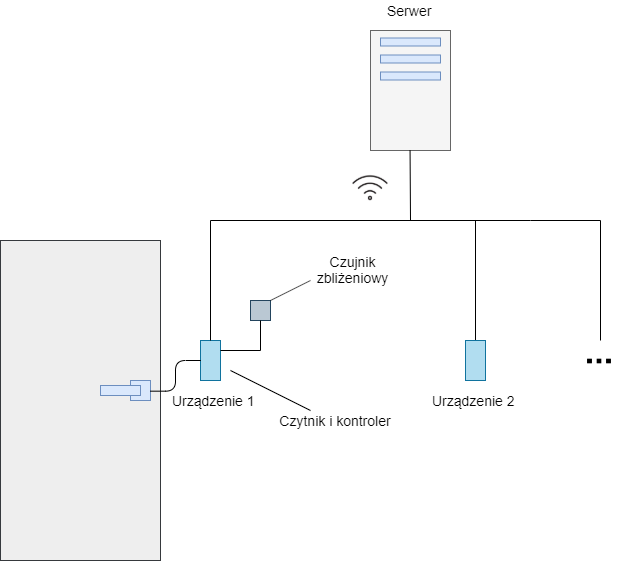
\includegraphics[width=\linewidth]{chapters/images/door2.png}
                \caption{Koncept systemu kontroli dostępu}
                \label{fig:door}
        \end{figure}

        Nadrzędnym celem systemu jest umożliwienie kontroli dostępu na terenie danego obiektu. Poświadczenie tożsamości (\textit{credentials}) stanowią karty RFID przyznawane użytkownikom systemu. Każda karta powiązana jest ze zbiorem zamków, w których zostanie z powodzeniem autoryzowana.

        \section{Działanie systemu}
                Poniżej w ogólny sposób opisano zakładany sposób działania systemu na podstawie scenariusza próby uzyskania dostępu przez użytkownika systemu.

                Kontroler zamka pozostaje uśpiony do momentu wykrycia ruchu w pobliżu przez czujnik ruchu. Po wybudzeniu, kontroler nawiązuje bezpieczne połączenie z serwerem autoryzacji, jednocześnie zasilając czytnik RFID oraz oczekując na zbliżenie do niego karty. Gdy karta zostanie zbliżona, kontroler przesyła odczytany z niej numer identyfikacyjny wraz z numerem identyfikacyjnym zamka do serwera. Na podstawie tych danych, serwer podejmuje decyzję, którą jest przyznanie bądź odmowa dostępu, a następnie przesyła informację zwrotną do kontrolera. Jeżeli podjęto decyzję o przyznaniu dostępu, kontroler wysyła sygnał otwarcia zamka oraz sygnalizuje powodzenie. Jeżeli podjęto decyzję o odmowie dostępu, kontroler sygnalizuje niepowodzenie. Diagram sekwencji obrazujący opisywany scenariusz przedstawiony jest na rysunku \ref{fig:sequence1}.

                \begin{figure}[]
                        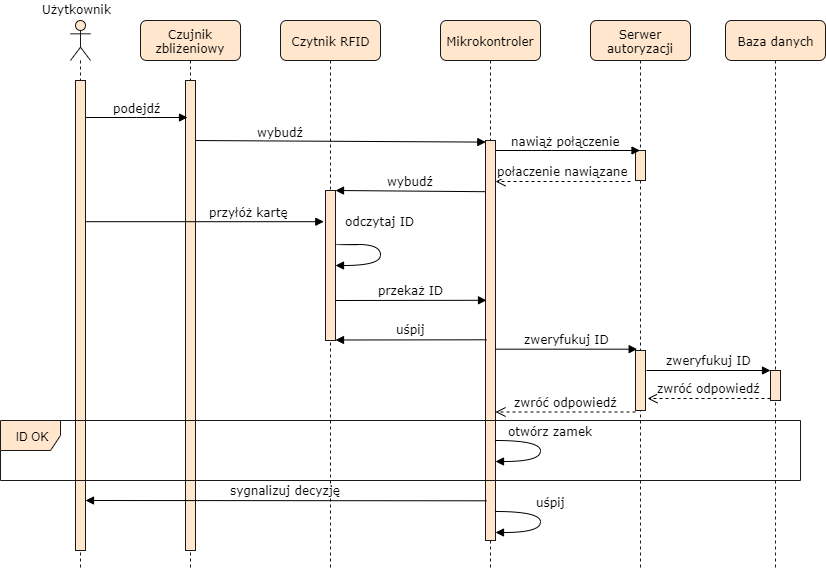
\includegraphics[width=\linewidth]{chapters/images/sequence1.png}
                        \caption{Diagram sekwencji ukazujący zasadę działania systemu}
                        \label{fig:sequence1}
                \end{figure}

                Niezależnie od rezultatu, wpis o próbie dostępu zostaje zapisany w bazie danych, skąd może być pobrany przez podsystem zarządzania w celu prezentacji danych administratorowi systemu.

        \section{Architektura systemu}

                W ramach systemu można wyodrębnić następujące podsystemy:
                \begin{enumerate}
                        \item Podsystem sterowania zamkiem,
                        \item Podsystem autoryzacji,
                        \item Podsystem zarządzania.
                \end{enumerate}

                Przedstawione wyżej podsystemy współistnieją w ramach dwóch komponentów sprzętowych. Są to:
                \begin{enumerate}
                        \item Komponent sterujący zamkiem (inaczej: kontroler, układ zamka),
                        \item Komponent serwera.
                \end{enumerate}

                Komponenty sprzętowe zostały krótko omówione w kolejnych punktach. Ogólna sprzętowa architektura systemu z podziałem na komponenty oraz przynależne im podsystemy przedstawiona została na rysunku \ref{fig:hl-arch}.

                \begin{figure}[]
                        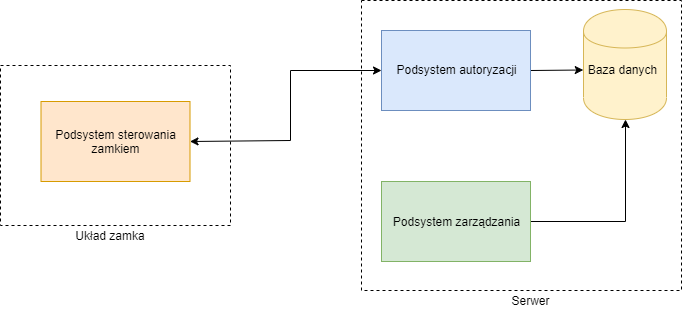
\includegraphics[width=\linewidth]{chapters/images/hl-arch3.png}
                        \caption{Architektura systemu}
                        \label{fig:hl-arch}
                \end{figure}

                \subsection{Komponent sterujący zamkiem}

                        Założono realizację następujących funkcjonalności w ramach komponentu sterującego zamkiem:
                        \begin{itemize}
                            \item Komunikacja bezprzewodowa z serwerem autoryzacji,
                            \item Komunikacja z pozostałymi komponentami podsystemu sterowania zamkiem (czujnik ruchu, czytnik RFID),
                            \item Kontrola przepływu sterowania,
                            \item Kontrola stanu zasilania komponentów podsystemu.
                        \end{itemize}

                        Komponent sterujący zamkiem składa się z mikrokontrolera, czujnika ruchu oraz czytnika RFID. Mikrokontroler odpowiada za sterowanie peryferiami, zarządza ich zasilaniem, inicjuje i przeprowadza bezprzewodową komunikację z serwerem i steruje samym zamkiem na podstawie otrzymanych od serwera danych. Podsystem sterowania zamkiem zlokalizowany jest w całości w tym komponencie (patrz rysunek \ref{fig:hl-arch}). Architektura układu zamka została przedstawiona na rysunku \ref{fig:lock-arch}. 

                        \begin{figure}
                                \centering
                                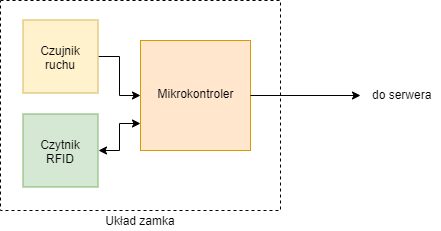
\includegraphics[width=0.7\textwidth]{chapters/images/lock.png}
                                \caption{Architektura układu zamka}
                                \label{fig:lock-arch}
                        \end{figure}

                \subsection{Serwer}
                        W ramach komponentu serwera działają dwa podsystemy funkcjonalne: podsystem autoryzacji, odpowiedzialny za podjęcie decyzji o przyznaniu lub odmowie dostępu na podstawie danych odebranych od podsystemu sterowania zamkiem, oraz podsystem zarządzania, odpowiedzialny za umożliwienie wygodnej konfiguracji systemu, oraz zbieranie i prezentację danych. Oba te systemy korzystają ze wspólnej bazy danych.

                        \subsubsection{Podsystem autoryzacji}
                                Zadaniem podsystemu autoryzacji jest podjęcie decyzji o przyznaniu bądź odmowie dostępu na podstawie otrzymanych danych. Podsystem komunikuje się z bazą danych w celu uzyskania informacji na temat autoryzowanych kart.

                                Założono realizację następujących funkcjonalności w ramach podsystemu autoryzacji:
                                \begin{itemize}
                                        \item Autoryzowanie kart w zamkach na podstawie otrzymanych od podsystemu sterowania zamkiem danych oraz zawartości bazy danych,
                                        \item Aktualizacja zawartości bazy danych o dokonane próby dostępu,
                                        \item Komunikacja z podsystemem sterowania zamkiem.
                                \end{itemize}

                        \subsubsection{Podsystem zarządzania}
                                Zadaniem podsystemu zarządzania jest umożliwienie użytkownikowi systemu wglądu do danych takich jak historia prób dostępu, zbiór zamków, kart oraz powiązań między nimi, oraz stan poszczególnych zamków. Dzięki niemu możliwa jest konfiguracja rozpoznawanych przez system kart, zamków oraz manualne przyznawanie dostępu poszczególnym identyfikatorom.

                                Podsystem zarządzania umożliwia następujące operacje:
                                \begin{itemize}
                                        \item Dodanie zamka,
                                        \item Usunięcie zamka,
                                        \item Dodanie karty wraz z przyznaniem jej dostępu do istniejącego zamka (lub też większej ich liczby),
                                        \item Usunięcie karty,
                                        \item Zablokowanie dostępu dla karty (bez usuwania jej z systemu),
                                        \item Przegląd archiwalnych prób dostępu,
                                        \item Podgląd parametrów zamka (stan baterii). \textbf{???}
                                \end{itemize}

                        \subsubsection{Baza danych}
                                Częścią komponentu serwera jest baza danych. Nie jest jednak konieczne, aby pozostawała ona fizycznie na tej samej maszynie. W przypadku całkowitego rozdzielenia serwera danych od serwera autoryzacji skalowalność systemu znacząco wzrośnie.

                                Baza danych przechowuje dane dotyczące poszczególnych kart i zamków zarejestrowanych w systemie, autoryzacji kart w zamkach oraz dokonanych w przeszłości prób dostępu, zarówno zakończonych sukcesem jak i porażką.

                                Schemat bazy danych przedstawiony został na rysunku \ref{fig:schema}

                                \begin{figure}
                                        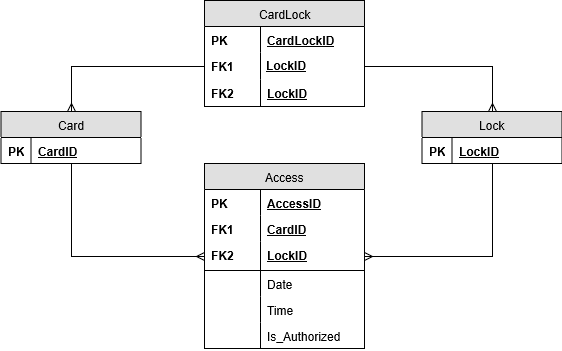
\includegraphics[width=\linewidth]{chapters/images/schema.png}
                                        \caption{Schemat bazy danych}
                                        \label{fig:schema}
                                \end{figure}

